\documentclass[14pt,a4paper]{scrreprt}

\usepackage{cmap}
\usepackage[T1]{fontenc} 
\usepackage[utf8]{inputenc}
\usepackage[english,russian]{babel}

\usepackage{caption}
\usepackage{subcaption}

\usepackage{float}

\usepackage{enumitem}

\usepackage{graphicx}
\usepackage{multirow}


\usepackage{pgfplots}
\pgfplotsset{compat=newest}
\usepgfplotslibrary{units}

\usepackage{longtable}

\usepackage{caption}
\captionsetup{labelsep=endash}
\captionsetup[figure]{name={Рисунок}}
\captionsetup[subtable]{labelformat=simple}
\captionsetup[subfigure]{labelformat=simple}
\renewcommand{\thesubtable}{\text{Таблица }\arabic{chapter}\text{.}\arabic{table}\text{.}\arabic{subtable}\text{ --}}
\renewcommand{\thesubfigure}{\text{Рисунок }\arabic{chapter}\text{.}\arabic{figure}\text{.}\arabic{subfigure}\text{ --}}


\usepackage{textcomp}

\usepackage{amsmath}
\usepackage{amsfonts}
\usepackage{array}

\usepackage{geometry}
\geometry{left=30mm}
\geometry{right=15mm}
\geometry{top=20mm}
\geometry{bottom=20mm}
\geometry{foot=1.7cm}

\usepackage{titlesec}
\titleformat{\section}
{\normalsize\bfseries}
{\thesection}
{1em}{}
\titlespacing*{\chapter}{0pt}{-30pt}{8pt}
\titlespacing*{\section}{\parindent}{*4}{*4}
\titlespacing*{\subsection}{\parindent}{*4}{*4}

% Маркировка для списков
\def\labelitemi{$\circ$}
\def\labelitemii{$*$}


\usepackage{setspace}
\onehalfspacing % Полуторный интервал

\frenchspacing
\usepackage{indentfirst} % Красная строка

\usepackage{titlesec}
\usepackage{xcolor}
% Названия глав
\titleformat{\section}{\normalsize\textmd}{\thesection}{1em}{}

\definecolor{gray35}{gray}{0.35}

\newcommand{\hsp}{\hspace{20pt}} % длина линии в 20pt

\titleformat{\chapter}[hang]{\Huge}{\textcolor{gray35}{\thechapter.}\hsp}{0pt}{\Huge\textmd}

\titleformat{\section}{\Large}{\textcolor{gray35}\thesection}{20pt}{\Large\textmd}
\titleformat{\subsection}{\Large}{\thesubsection}{20pt}{\Large\textmd}
\titleformat{\subsubsection}{\normalfont\textmd}{}{0pt}{}

% Настройки введения

\addtocontents{toc}{\setcounter{tocdepth}{2}}
\addtocontents{toc}{\setcounter{secnumdepth}{1}}

\usepackage{tocloft,lipsum,pgffor}

\addtocontents{toc}{~\hfill\textnormal{Страница}\par}

\renewcommand{\cftpartfont}{\normalfont\textmd}

\addto\captionsrussian{\renewcommand{\contentsname}{Содержание}}
\renewcommand{\cfttoctitlefont}{\Huge\textmd}

\renewcommand{\cftchapfont}{\normalfont\normalsize}
\renewcommand{\cftsecfont}{\normalfont\normalsize}
\renewcommand{\cftsubsecfont}{\normalfont\normalsize}
\renewcommand{\cftsubsubsecfont}{\normalfont\normalsize}

\renewcommand{\cftchapleader}{\cftdotfill{\cftdotsep}}

\usepackage{listings}
\usepackage{xcolor}

\usepackage[pdftex]{hyperref} % Гиперссылки
\hypersetup{hidelinks}

% Листинги 
\usepackage{listings}

\definecolor{darkgray}{gray}{0.15}

\definecolor{teal}{rgb}{0.25,0.88,0.73}
\definecolor{gray}{rgb}{0.5,0.5,0.5}
\definecolor{b-red}{rgb}{0.88,0.25,0.41}
\definecolor{royal-blue}{rgb}{0.25,0.41,0.88}

\usepackage{listings}
\lstset{
	aboveskip=3mm,
	belowskip=3mm,
	frame=tb,
	frame=single,
	basicstyle=\footnotesize\ttfamily,
	numberstyle=\tiny\color{gray},
	keywordstyle=\color{royal-blue},
	commentstyle=\color{gray35},
	stringstyle=\color{b-red},
	numbers=left,
	numbersep=5pt,
	numberstyle=\tiny,
	showstringspaces=false, 
	captionpos=t,
	tabsize=4,
	language=Lisp
}

% какой то сложный кусок со стак эксчейндж для квадратных скобок
\makeatletter
\newenvironment{sqcases}{%
	\matrix@check\sqcases\env@sqcases
}{%
	\endarray\right.%
}
\def\env@sqcases{%
	\let\@ifnextchar\new@ifnextchar
	\left\lbrack
	\def\arraystretch{1.2}%
	\array{@{}l@{\quad}l@{}}%
}
\makeatother

% и для матриц
\makeatletter
\renewcommand*\env@matrix[1][\arraystretch]{%
	\edef\arraystretch{#1}%
	\hskip -\arraycolsep
	\let\@ifnextchar\new@ifnextchar
	\array{*\c@MaxMatrixCols c}}
\makeatother


\begin{document}

\begin{titlepage}
	
	\newgeometry{left=2cm, right=2cm, top=2.5cm, bottom=2.5cm}
	\fontsize{12pt}{12pt}\selectfont
	
	\noindent \begin{minipage}{0.13\textwidth}
		
\includegraphics[width=\linewidth]{assets/bmstu-logo.png}
	\end{minipage}
	\noindent\begin{minipage}{0.85\textwidth}\centering
		\textbf{\textsc{Министерство науки и высшего образования Российской Федерации}}\\
		\textbf{\textsc{Федеральное государственное бюджетное образовательное 	учреждение высшего образования}}\\
		\textbf{\textsc{Московский государственный технический университет имени 	Н.Э.~Баумана}}\\
		\textbf{\textsc{(национальный исследовательский университет)}}\\
		\textbf{\textsc{(МГТУ им. Н.Э. Баумана)}}\\
	\end{minipage}
	
	\noindent\rule{18cm}{1.5pt}
	
	\vspace{8mm}
	
	\noindent\textnormal{ФАКУЛЬТЕТ}\hspace{5mm} \underline{\textnormal{~~~~~~~~~~~~~~~~~~«Информатика и системы управления»~~~~~~~~~~~~~~~~~~}} \newline\newline
	\textnormal{КАФЕДРА}\hspace{5mm} \underline{\textnormal{~~«Программное обеспечение ЭВМ и информационные технологии»~~}}
	\newline\newline
	\textnormal{НАПРАВЛЕНИЕ ПОДГОТОВКИ}\hspace{5mm} \underline{\textnormal{~~~~~~«09.03.04 Программная инженерия»~~~~~~~~}}
	
	\vspace{2.5cm}
	
	\begin{center}
		\Large\textbf{\textsc{ОТЧЕТ}}\\
		\Large\textbf{\textsc{ПО ЛАБОРАТОРНОЙ РАБОТЕ №18}}\\
	\end{center}
	
	\vspace{1cm}
	
	\noindent\textnormal{Название:} \hspace{15mm} \underline{\textnormal{~~~~~~Формирование и модификация списков на Prolog~~~~~~~}}\noindent
	
	\vspace{1.3cm}
	
	\noindent\textnormal{Дисциплина:} \hspace{10mm} \underline{\textnormal{~~~~~~Функциональное и логическое программирование~~~~~~}}\noindent
	
	\vspace{1.5cm}
	
	\noindent\textnormal{Студент} \hspace{17mm}
	\underline{\textnormal{{~~~~ИУ7-64Б~~~}}}
	\hspace{20mm}
	\underline{\textnormal{\hphantom{~~~~~~~~~~~~~~~~~~~~~~~~~~~}}} \hspace{14mm}
	\underline{\textnormal{~~~С. Д. Параскун~~~}}
	
	\vspace{2mm}
	\noindent\textnormal{\hphantom{Студент}} \hspace{23mm}\noindent
	\fontsize{8pt}{8pt}
	\textnormal{Группа}\hspace{40mm}\textnormal{Подпись, дата} \hspace{30mm}\noindent\textnormal{И. О. Фамилия}
	
	\vspace{0.5cm}
	
	\fontsize{12pt}{12pt}\selectfont
	\noindent\textnormal{Преподаватель} \hspace{52mm}
	\underline{\textnormal{\hphantom{~~~~~~~~~~~~~~~~~~~~~~~~~~~}}} \hspace{14mm}
	\noindent\underline{\textnormal{~~Н. Б. Толпинская~~}}
	
	\vspace{2mm}
	\noindent\textnormal{\hphantom{Студент}} \hspace{17mm}\noindent
	\fontsize{8pt}{8pt}
	\hphantom{Группа}\hspace{43mm}\textnormal{Подпись, дата} \hspace{30mm}\noindent\textnormal{И. О. Фамилия}
	
	\vspace{0.5cm}
	
	\fontsize{12pt}{12pt}\selectfont
	\noindent\textnormal{Преподаватель} \hspace{52mm}
	\underline{\textnormal{\hphantom{~~~~~~~~~~~~~~~~~~~~~~~~~~~}}} \hspace{14mm}
	\noindent\underline{\textnormal{~~Ю. В. Строганов~~}}
	
	\vspace{2mm}
	\noindent\textnormal{\hphantom{Студент}} \hspace{17mm}\noindent
	\fontsize{8pt}{8pt}
	\hphantom{Группа}\hspace{43mm}\textnormal{Подпись, дата} \hspace{30mm}\noindent\textnormal{И. О. Фамилия}
	
	\vspace{1cm}
	
	\fontsize{12pt}{12pt}\selectfont
	
	\begin{center}
		\vfill
		Москва, ~\the\year
		~г.
	\end{center}
	\restoregeometry

\end{titlepage}


\thispagestyle{empty}

\chapter{Теоретические вопросы}

\section{Синтаксическая форма и хранение программы в памяти}

В Lisp программа синтаксически представлена в форме S-выражений. Особенностью является единая форма фиксации (отсутствие разделения на программу и данные). И то, и другое представляется списочной структурой, имеющей одинаковую форму. Благодаря такому подходу возможно изменение кода программы при обработке данных.

Так как программа имеет вид S-выражения, в памяти она представлена либо как атом (5 указателей, которыми представляется атом в памяти), либо как списковая ячейка (2 указателя, бинарный узел).

\section{Трактовка элементов списка}

При обработке списков первый элемент воспринимается интерпретатором как название функции, все остальные -- ее аргументы. Количество элементов, не считая первого -- названия функции, должно совпадать с количеством входных аргументов указанной функции.

В случае если перед скобкой стоит блокировка (` или '), вычисления не производятся, и результатом является все, что стоит после блокировки.

\begin{lstlisting}
	(defun mult (a b c) (* a b c))
	(mult 1 2 3) ; => 6; mult - name of func; 1, 2, 3 - arguments
	(mult 0 1 2 3) ; => error - invalid number of arguments
	'(eval func 3) ; => (eval func 3)
\end{lstlisting}
\newpage

\section{Порядок реализации программы}

\begin{enumerate}
	\item Ожидает ввода S-выражения.
	\item Передает введенное S-выражение функции eval.
	\item Выводит полученный результат.
\end{enumerate}

\begin{figure}[H]
	\begin{center}
		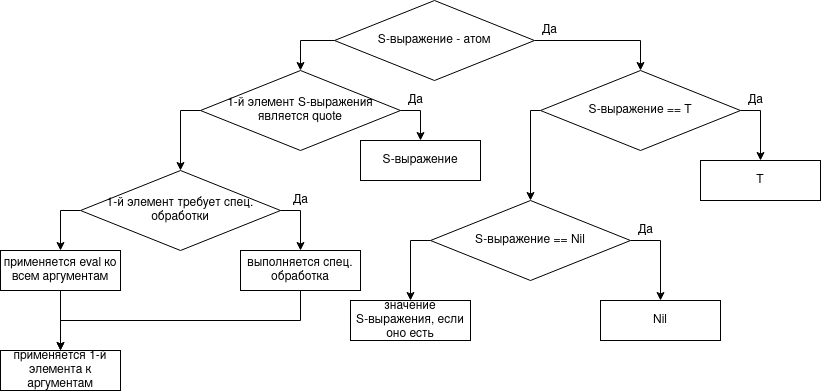
\includegraphics[scale=0.5]{assets/scheme.png}
	\end{center}
	\caption{Диаграмма работы функции eval}
\end{figure}


\section{Способы определения функции}

\begin{enumerate}
	\item С помощью lambda. После ключевого слова указывается лямбда-список и тело функции. 
	\begin{lstlisting}
	(lambda (x y) (+ x y))
	\end{lstlisting}
	Для применения используются лямбда-выражения.
	\begin{lstlisting}
	((lambda (x y) (+ x y)) 1 2)
	\end{lstlisting}
	\item С помощью defun. Используется для неоднократного применения функции (в том числе рекурсивного вызова).
	\begin{lstlisting}
	(defun sum (x y) (+ x y))
	(sum 1 2)
	\end{lstlisting}
\end{enumerate}

\end{document}